\documentclass[letter,11pt]{article}

\usepackage[spanish,es-nodecimaldot]{babel}
\usepackage[utf8]{inputenc}

\usepackage{lmodern}
\usepackage[T1]{fontenc}
\usepackage{textcomp}

\usepackage{framed}
\usepackage[svgnames]{xcolor}
\colorlet{shadecolor}{Gainsboro!50}

\usepackage[shortlabels]{enumitem}
\usepackage{graphicx}
\usepackage{pstricks}

\usepackage{anysize}
\marginsize{3cm}{2cm}{2cm}{3cm}

\usepackage{siunitx}
\usepackage{amsmath}
\usepackage{array}
\usepackage{alltt}

\usepackage{fancyhdr}
\usepackage{lastpage}
\pagestyle{fancy}
\fancyhf{}
\fancyhead[LE,RO]{Física Básica III}
\fancyfoot[CO,CE]{\thepage\ de \pageref{LastPage}}

\special{papersize=215.9mm,279.4mm}

\usepackage[
    pdfauthor={Carlos Eduardo Caballero Burgoa},%
    pdftitle={Física Básica III},%
    pdfsubject={Tarea},%
    colorlinks,%
    citecolor=black,%
    filecolor=black,%
    linkcolor=black,%
    urlcolor=black,
    breaklinks]{hyperref}
\usepackage{breakurl}

\newcommand{\blankpage}{
\newpage
\thispagestyle{empty}
\mbox{}
\newpage
}

\renewcommand{\arraystretch}{1.2}
\newcommand{\pvec}[1]{\vec{#1}\mkern2mu\vphantom{#1}}

\begin{document}

\begin{center}
    {\Large \bf{\underline{Tarea}}}
\end{center}
\vspace{0.5cm}

\textbf{21.97.}
Dos varillas delgadas de longitud $L$ están a lo largo del eje $x$, una entre
$x=\frac{1}{2}a$ y $x=\frac{1}{2}a+L$, y la otra entre
$x=-\frac{1}{2}a$ y $x=-\frac{1}{2}a-L$. Cada varilla tiene carga positiva
$Q$ distribuida uniformemente en toda su longitud.

\begin{figure}[!h]
\centering
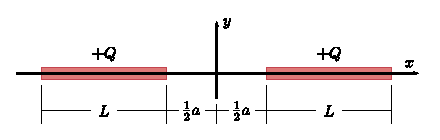
\includegraphics[scale=1.50]{resources/f1.eps}
\end{figure}

\begin{enumerate}[a)]
\item Calcule el campo eléctrico producido por la segunda varilla en
puntos a lo largo del eje x positivo.

\item Demuestre que la magnitud de la fuerza que ejerce una varilla sobre
la otra es:

\begin{equation*}
    F = \frac{Q^2}{4\pi\epsilon_0 L^2}\,ln\left[\frac{(a+L)^2}{a(a+2L)}\right]
\end{equation*}
\vspace{0.20cm}

\item Demuestre que si $a \gg L$, la magnitud de esta fuerza se reduce a:

\begin{equation*}
    F = \frac{Q^2}{4\pi\epsilon_0 a^2}
\end{equation*}
\vspace{0.20cm}

\emph{Sugerencia}: Use la expansión:
$ln(1+z)=z-\frac{1}{2}z^2+\frac{1}{3}z^3-\cdots$, válida para $|z|\ll 1$.
Considere \emph{todas} las expansiones al menos hasta el orden
$\frac{L^2}{a^2}$. Interprete este resultado.
\end{enumerate}
\vspace{0.75cm}

\textbf{\underline{Solución}:} \\

\textbf{a)}
\begin{figure}[!h]
\centering
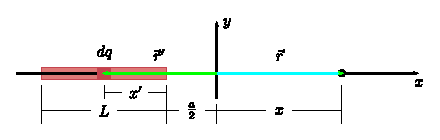
\includegraphics[scale=1.50]{resources/f2.eps}
\end{figure}
\vspace{0.20cm}

Los vectores de posición de las cargas son:

\begin{equation*}
    \vec{r} = x\hat{u}_x
\end{equation*}
\begin{equation*}
    \pvec{r}' = -\left(\frac{a}{2}+x'\right)\hat{u}_x
\end{equation*}
\vspace{0.20cm}

Considerando la distribución homogénea de la carga:

\begin{equation*}
    \lambda = \frac{dq}{dx'}
\end{equation*}
\vspace{0.20cm}

El campo eléctrico es:

\begin{equation*}
    \vec{E} = \int_Q\frac{1}{4\pi\epsilon_0}dq
              \frac{(\vec{r}-\pvec{r}')}{|\vec{r}-\pvec{r}'|^3}
\end{equation*}
\vspace{0.20cm}

Reemplazando $dq=\lambda dx'$ y los vectores de posición $\vec{r}$ y
$\pvec{r}'$:

\begin{equation*}
\begin{split}
    \vec{E} &= \frac{1}{4\pi\epsilon_0}\int_0^L\lambda dx'
               \frac{(x\hat{u}_x+\frac{a}{2}\hat{u}_x+x'\hat{u}_x)}
               {|x\hat{u}_x+\frac{a}{2}\hat{u}_x+x'\hat{u}_x|^3}\\
            &= \frac{\lambda}{4\pi\epsilon_0}\int_0^L dx'
               \frac{(x+\frac{a}{2}+x')}{(x+\frac{a}{2}+x')^3}
               \hat{u}_x\\
            &= \frac{\lambda}{4\pi\epsilon_0}\int_0^L
               \frac{dx'}{(x+\frac{a}{2}+x')^2}\hat{u}_x
\end{split}
\end{equation*}
\vspace{0.20cm}

Realizando un cambio de variable para resolver la integral:

\begin{equation*}
    u = x+\frac{a}{2}+x'
\end{equation*}
\begin{equation*}
    du = dx'
\end{equation*}
\vspace{0.20cm}

Por tanto:

\begin{equation*}
    \int\frac{du}{u^2} = \int u^{-2}du
                       = \frac{u^{-2+1}}{-2+1}
                       = \frac{u^{-1}}{-1}
                       = -\frac{1}{u}
\end{equation*}
\vspace{0.20cm}

Reemplazando en la función original:

\begin{equation*}
\begin{split}
    \vec{E} &= \frac{\lambda}{4\pi\epsilon_0}
               \left(-\frac{1}{x+\frac{a}{2}+x'}\Biggr|_0^L\right)
               \hat{u}_x\\
            &= \frac{\lambda}{4\pi\epsilon_0}
               \left(-\frac{1}{x+\frac{a}{2}+L}+
               \frac{1}{x+\frac{a}{2}}\right)\hat{u}_x\\
            &= \frac{\lambda}{4\pi\epsilon_0}
               \left(\frac{1}{x+\frac{a}{2}}-
               \frac{1}{x+\frac{a}{2}+L}\right)\hat{u}_x
\end{split}
\end{equation*}
\vspace{0.20cm}

Reemplazando $\lambda=Q/L$:

\begin{equation*}
\begin{split}
    \vec{E} &= \frac{1}{4\pi\epsilon_0}\frac{Q}{L}
               \left(\frac{2}{2x+a}-\frac{2}{2x+a+2L}\right)\hat{u}_x\\
            &= \frac{1}{2\pi\epsilon_0}\frac{Q}{L}
               \left(\frac{1}{2x+a}-\frac{1}{2x+a+2L}\right)\hat{u}_x
\end{split}
\end{equation*}
\vspace{0.20cm}

\textbf{b)}
\begin{figure}[!h]
\centering
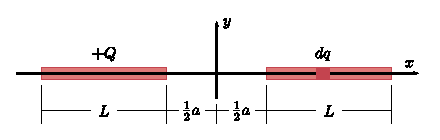
\includegraphics[scale=1.50]{resources/f3.eps}
\end{figure}
\vspace{0.20cm}

La fuerza ejercida por la varilla sobre un diferencial $dq$ en el eje $x$ es:

\begin{equation*}
    \vec{F} = \int_Q\vec{E}\,dq
            = \int_Q\frac{1}{2\pi\epsilon_0}\frac{Q}{L}
              \left(\frac{1}{2x+a}-\frac{1}{2x+a+2L}\right)dq\,\hat{u}_x
\end{equation*}
\vspace{0.20cm}

Reemplazando $dq=\lambda dx$:

\begin{equation*}
\begin{split}
    \vec{F} &= \int_{\frac{a}{2}}^{\frac{a}{2}+L}\frac{1}{2\pi\epsilon_0}
               \frac{Q}{L}\left(\frac{1}{2x+a}-\frac{1}{2x+a+2L}\right)
               \lambda dx\,\hat{u}_x\\
            &= \frac{1}{2\pi\epsilon_0}\frac{\lambda Q}{L}
               \int_{\frac{a}{2}}^{\frac{a}{2}+L}
               \frac{1}{2x+a}-\frac{1}{2x+a+2L}dx\,\hat{u}_x
\end{split}
\end{equation*}
\vspace{0.20cm}

Reemplazando $\lambda=Q/L$:

\begin{equation*}
    \vec{F} = \frac{1}{2\pi\epsilon_0}\frac{Q^2}{L^2}
              \left(\int_{\frac{a}{2}}^{\frac{a}{2}+L}\frac{dx}{2x+a}-
              \int_{\frac{a}{2}}^{\frac{a}{2}+L}\frac{dx}{2x+a+2L}\right)
              \hat{u}_x
\end{equation*}
\vspace{0.20cm}

Realizando un cambio de variable para resolver la integral:

\begin{equation*}
    u = 2x+a
\end{equation*}
\begin{equation*}
    du = 2\,dx
\end{equation*}
\vspace{0.20cm}

Por tanto:

\begin{equation*}
    \int\frac{1}{2}\frac{du}{u} = \frac{1}{2}\int\frac{du}{u}
                                = \frac{ln\,u}{2}
\end{equation*}
\vspace{0.20cm}

Reemplazando en la función original:

\begin{equation*}
\begin{split}
    \vec{F} &= \frac{1}{2\pi\epsilon_0}\frac{Q^2}{L^2}\frac{1}{2}
               \left(ln\,(2x+a)\Biggr|_{\frac{a}{2}}^{\frac{a}{2}+L}-
               ln\,(2x+a+2L)\Biggr|_{\frac{a}{2}}^{\frac{a}{2}+L}\right)
               \hat{u}_x\\
            &= \frac{1}{4\pi\epsilon_0}\frac{Q^2}{L^2}
               (ln\,(2(\frac{a}{2}+L)+a)-ln\,(2(\frac{a}{2})+a)\\
            &- ln\,(2(\frac{a}{2}+L)+a+2L)+ln\,(2(\frac{a}{2})+a+2L))\hat{u}_x\\
            &= \frac{1}{4\pi\epsilon_0}\frac{Q^2}{L^2}
               \left(ln\,(2a+2L)-ln\,(2a)-
               ln\,(2a+4L)+ln\,(2a+2L)\right)\hat{u}_x\\
            &= \frac{1}{4\pi\epsilon_0}\frac{Q^2}{L^2}\,
               ln\,\left(\frac{(2a+2L)(2a+2L)}{2a(2a+4L)}\right)\hat{u}_x\\
            &= \frac{1}{4\pi\epsilon_0}\frac{Q^2}{L^2}\,
               ln\,\left(\frac{4(a+L)^2}{4a(a+2L)}\right)\hat{u}_x\\
            &= \frac{1}{4\pi\epsilon_0}\frac{Q^2}{L^2}\,
              ln\,\left(\frac{(a+L)^2}{a(a+2L)}\right)\hat{u}_x
\end{split}
\end{equation*}
\vspace{0.20cm}

\textbf{c)}\\

Transformando la función a expresiones tipo $1+\frac{L}{a}$:

\begin{equation*}
    (a+L) = \frac{a}{a}(a+L)
          = a\left(1+\frac{L}{a}\right)
\end{equation*}
\begin{equation*}
    (a+2L) = \frac{a}{a}(a+2L)
           = a\left(1+\frac{2L}{a}\right)
\end{equation*}
\vspace{0.20cm}

Reemplazando en la función original:

\begin{equation*}
\begin{split}
    \vec{F} &= \frac{1}{4\pi\epsilon_0}\frac{Q^2}{L^2}\,ln\,\left(
               \frac{a^2(1+\frac{L}{a})^2}{a^2(1+\frac{2L}{a})}\right)
               \hat{u}_x\\
            &= \frac{1}{4\pi\epsilon_0}\frac{Q^2}{L^2}\,ln\,\left(
               \frac{(1+\frac{L}{a})^2}{(1+\frac{2L}{a})}\right)\hat{u}_x\\
            &= \frac{1}{4\pi\epsilon_0}\frac{Q^2}{L^2}
               \left(2\,ln\,\left(1+\frac{L}{a}\right)-
               ln\,\left(1+\frac{2L}{a}\right)\right)\hat{u}_x
\end{split}
\end{equation*}
\vspace{0.20cm}

Sabiendo que para $|z|\ll 1$:

\begin{equation*}
    ln\,(1+z) = z-\frac{1}{2}z^2+\frac{1}{3}z^3-\cdots
\end{equation*}
\vspace{0.20cm}

Y considerando $a \gg L$:

\begin{equation*}
\begin{split}
    \vec{F} &= \frac{1}{4\pi\epsilon_0}\frac{Q^2}{L^2}
               \left(2\,\left(\frac{L}{a}-\frac{1}{2}
               \left(\frac{L}{a}\right)^2\right)-
               \left(\frac{2L}{a}-\frac{1}{2}\left(\frac{2L}{a}\right)^2
               \right)\right)\hat{u}_x\\
            &= \frac{1}{4\pi\epsilon_0}\frac{Q^2}{L^2}
               \left(2\,\left(\frac{L}{a}-\frac{L^2}{2a^2}\right)-
               \left(\frac{2L}{a}-\frac{4L^2}{2a^2}\right)\right)\hat{u}_x\\
            &= \frac{1}{4\pi\epsilon_0}\frac{Q^2}{L^2}
               \left(2\,\left(\frac{2aL-L^2}{2a^2}\right)-
               \left(\frac{4aL-4L^2}{2a^2}\right)\right)\hat{u}_x\\
            &= \frac{1}{4\pi\epsilon_0}\frac{Q^2}{L^2}
               \left(\left(\frac{4aL-2L^2}{2a^2}\right)-
               \left(\frac{4aL-4L^2}{2a^2}\right)\right)\hat{u}_x\\
            &= \frac{1}{4\pi\epsilon_0}\frac{Q^2}{L^2}
               \left(\frac{4aL-2L^2-4aL+4L^2}{2a^2}\right)\hat{u}_x\\
            &= \frac{1}{4\pi\epsilon_0}\frac{Q^2}{L^2}
               \left(\frac{2L^2}{2a^2}\right)\hat{u}_x\\
            &= \frac{1}{4\pi\epsilon_0}\frac{Q^2}{a^2}\hat{u}_x
\end{split}
\end{equation*}
\vspace{0.20cm}

\end{document}

